\documentclass{standalone}
\usepackage{pgfplots}


\begin{document}

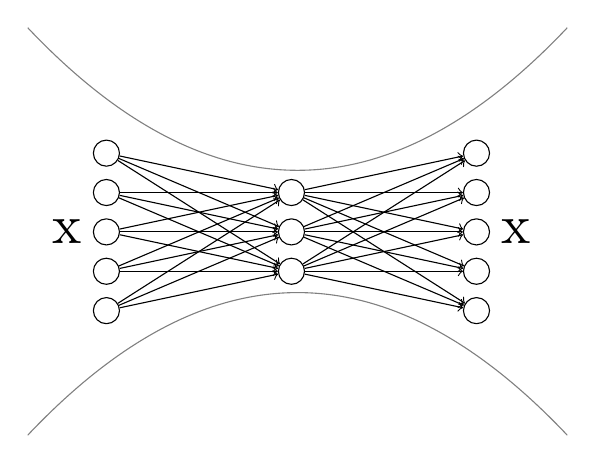
\begin{tikzpicture}
\begin{axis}[xmax=1,xmin=-1,ymax=1, samples=200, hide axis]
  \addplot[domain=-1:1, gray] (x, 0.7*x*x+0.3);
  \addplot[domain=-1:1, gray] (x, -0.7*x*x-0.3);
\end{axis}

\node[scale=2] at (0.5,3.1) {x};
\node[scale=2] at (6.2,3.1) {x};

\node[draw, circle, minimum size=0.2cm] (i1) at (1, 1+3.1) {};
\node[draw, circle, minimum size=0.2cm] (i2) at (1, 0.5+3.1) {};
\node[draw, circle, minimum size=0.2cm] (i3) at (1, 0+3.1) {};
\node[draw, circle, minimum size=0.2cm] (i4) at (1, -0.5+3.1) {};
\node[draw, circle, minimum size=0.2cm] (i5) at (1, -1+3.1) {};

\node[draw, circle, minimum size=0.2cm] (h1) at (3.35, 0.5+3.1) {};
\node[draw, circle, minimum size=0.2cm] (h2) at (3.35, 0+3.1) {};
\node[draw, circle, minimum size=0.2cm] (h3) at (3.35, -0.5+3.1) {};

\node[draw, circle, minimum size=0.2cm] (o1) at (5.7, 1+3.1) {};
\node[draw, circle, minimum size=0.2cm] (o2) at (5.7, 0.5+3.1) {};
\node[draw, circle, minimum size=0.2cm] (o3) at (5.7, 0+3.1) {};
\node[draw, circle, minimum size=0.2cm] (o4) at (5.7, -0.5+3.1) {};
\node[draw, circle, minimum size=0.2cm] (o5) at (5.7, -1+3.1) {};

% input -> hidden
\draw [->] (i1) edge (h1) (i1) edge (h2) (i1) edge (h3);
\draw [->] (i2) edge (h1) (i2) edge (h2) (i2) edge (h3);
\draw [->] (i3) edge (h1) (i3) edge (h2) (i3) edge (h3);
\draw [->] (i4) edge (h1) (i4) edge (h2) (i4) edge (h3);
\draw [->] (i5) edge (h1) (i5) edge (h2) (i5) edge (h3);

% hidden -> output
\draw [<-] (o1) edge (h1) (o1) edge (h2) (o1) edge (h3);
\draw [<-] (o2) edge (h1) (o2) edge (h2) (o2) edge (h3);
\draw [<-] (o3) edge (h1) (o3) edge (h2) (o3) edge (h3);
\draw [<-] (o4) edge (h1) (o4) edge (h2) (o4) edge (h3);
\draw [<-] (o5) edge (h1) (o5) edge (h2) (o5) edge (h3);

\end{tikzpicture}

\end{document}